\documentclass{article}



\usepackage[utf8]{inputenc}
\usepackage{longtable}
\usepackage{authblk}
\usepackage{adjustbox}

\usepackage{natbib}





\title{Indice De Desarrollo Humano en Colombia}
% autores
\renewcommand\Authand{ y }
\author[]{\normalsize Juan Victor Figueroa Mijares}

\affil[,]{\small  Facultad de Ingenieria,\\ 

Universidad de los Andes\\
\texttt{{jv.figueroa10}@uniandes.edu.co}}

\date{30 de Junio de 2018}
\usepackage{Sweave}
\begin{document}
\Sconcordance{concordance:ProyectoFinalJV.tex:ProyectoFinalJV.Rnw:%
1 52 1 1 9 2 1 1 4 15 0 1 3 4 1 1 15 1 5 6 1 1 12 1 3 2 1 1 8 13 0 1 4 %
12 1 1 8 12 0 1 4 7 1 1 10 14 0 1 3 9 1 1 4 1 2 13 1 1 2 7 1 1 6 2 1 1 %
4 31 0 1 2 19 1}


\maketitle

\begin{abstract}


Este es mi primer trabajo en exploracion y modelamiento de indices usando LATEX. Este trabajo lo he hecho bajo la filosofia de trabajo replicable.

\end{abstract}


\section*{Introduccion}


Aqui les presento mi investigacion sobre diversos indices sociales en el mundo. Los indices los consegui de wikipedia,espero que les gusten mucho. 

\clearpage

\section{Exploracion Univariada}\label{univariada}

  En esta seccion exploro cada indice.

  Este es el comportamiento de las variables a estudiar.    Veamos su tabla de frecuencias:




% Table created by stargazer v.5.2.2 by Marek Hlavac, Harvard University. E-mail: hlavac at fas.harvard.edu
% Date and time: Sat, Jul 07, 2018 - 18:46:45
\begin{table}[!htbp] \centering 
  \caption{Medias Estadisticas} 
  \label{Status} 
\begin{tabular}{@{\extracolsep{5pt}}lccccc} 
\\[-1.8ex]\hline 
\hline \\[-1.8ex] 
Statistic & \multicolumn{1}{c}{N} & \multicolumn{1}{c}{Min} & \multicolumn{1}{c}{Median} & \multicolumn{1}{c}{Max} & \multicolumn{1}{c}{Mean} \\ 
\hline \\[-1.8ex] 
IDH & 32 & 0.691 & 0.804 & 0.879 & 0.802 \\ 
Poblaci..n.Cabecera & 32 & 13,090 & 717,197 & 10,070,801 & 1,196,730.000 \\ 
Poblaci..n.Resto & 32 & 21,926 & 268,111.5 & 1,428,858 & 360,590.300 \\ 
Poblaci..n.Total & 32 & 43,446 & 1,028,429 & 10,985,285 & 1,557,320.000 \\ 
\hline \\[-1.8ex] 
\end{tabular} 
\end{table} 

\begin{figure}[h]
\centering

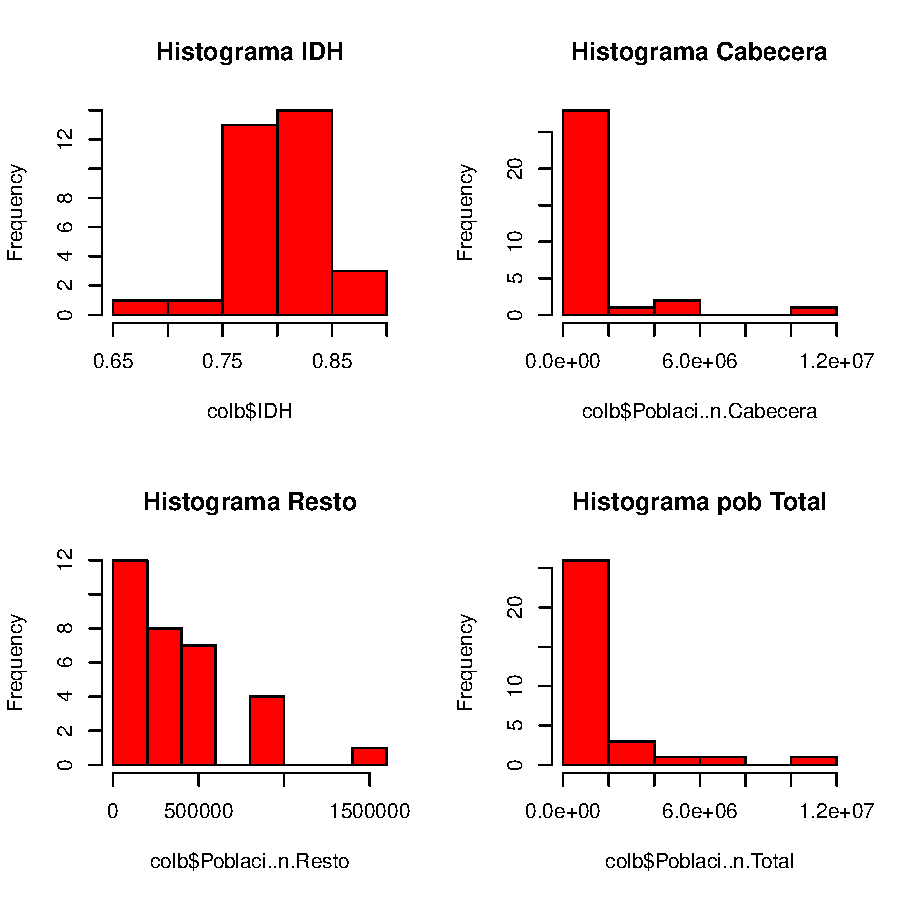
\includegraphics{ProyectoFinalJV-histogramas}

\caption{Histogramas variables de interes}
\label{histog}
\end{figure}

Dado el sesgo de las poblaciones, podemos trasformaslas aplicando el logaritmo para que se acerquen a la normalidad. 

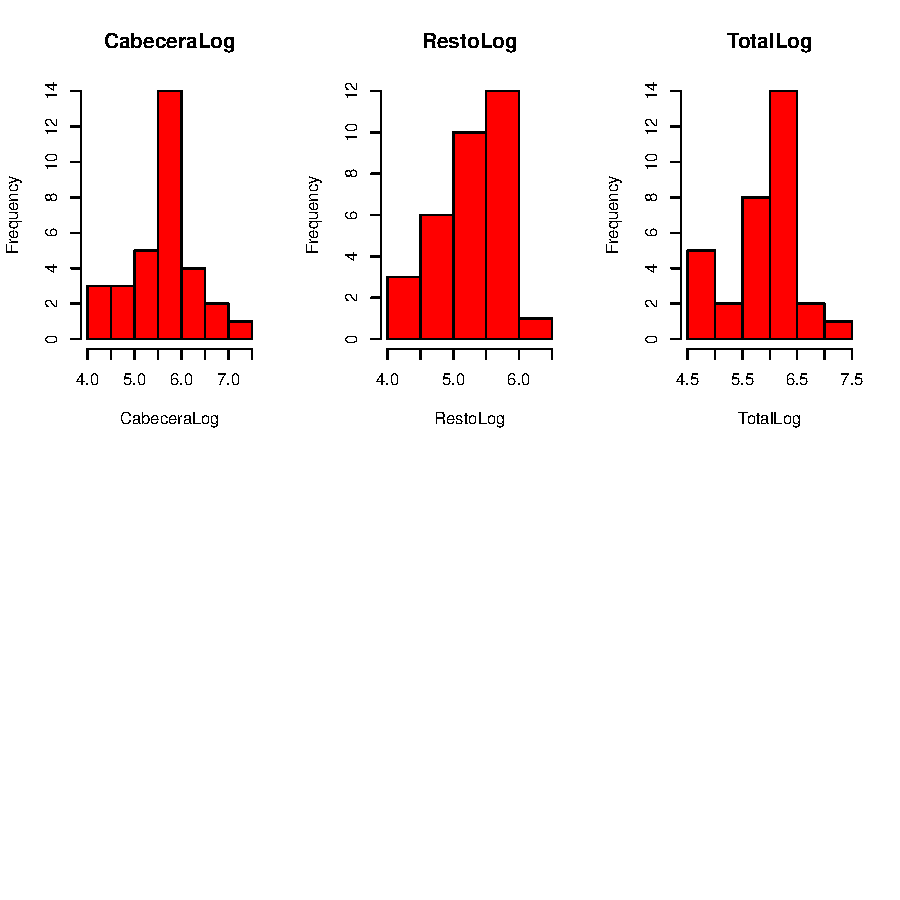
\includegraphics{ProyectoFinalJV-HistogramasAjustados}



% Table created by stargazer v.5.2.2 by Marek Hlavac, Harvard University. E-mail: hlavac at fas.harvard.edu
% Date and time: Sat, Jul 07, 2018 - 18:46:51
\begin{table}[!htbp] \centering 
  \caption{Medidas estadisticas datos Transformados} 
  \label{stats1} 
\begin{tabular}{@{\extracolsep{5pt}}lccccc} 
\\[-1.8ex]\hline 
\hline \\[-1.8ex] 
Statistic & \multicolumn{1}{c}{N} & \multicolumn{1}{c}{Min} & \multicolumn{1}{c}{Median} & \multicolumn{1}{c}{Max} & \multicolumn{1}{c}{Mean} \\ 
\hline \\[-1.8ex] 
Cabecera.Ajustada & 32 & 9.480 & 13.483 & 16.125 & 13.034 \\ 
Resto.Ajustada & 32 & 9.995 & 12.499 & 14.172 & 12.293 \\ 
\hline \\[-1.8ex] 
\end{tabular} 
\end{table} 





\clearpage

\section{Exploracion Bivariada}

En este trabajo estamos interesados en el impacto de los otros indices en el nivel de IDH. Veamos las relaciones bivariadas que tiene esta variable con todas las demas:


% Table created by stargazer v.5.2.2 by Marek Hlavac, Harvard University. E-mail: hlavac at fas.harvard.edu
% Date and time: Sat, Jul 07, 2018 - 18:46:51
\begin{table}[!htbp] \centering 
  \caption{Correlacion del IDH con las poblaciones} 
  \label{corIDH} 
\begin{tabular}{@{\extracolsep{5pt}} ccc} 
\\[-1.8ex]\hline 
\hline \\[-1.8ex] 
Poblaci..n.Cabecera & Poblaci..n.Resto & Poblaci..n.Total \\ 
\hline \\[-1.8ex] 
$0.487$ & $0.177$ & $0.424$ \\ 
\hline \\[-1.8ex] 
\end{tabular} 
\end{table} 





La correlacion entre las variables independientes

% Table created by stargazer v.5.2.2 by Marek Hlavac, Harvard University. E-mail: hlavac at fas.harvard.edu
% Date and time: Sat, Jul 07, 2018 - 18:46:51
\begin{table}[!htbp] \centering 
  \caption{Correlacion entre variables independientes} 
  \label{corrTableX} 
\begin{tabular}{@{\extracolsep{5pt}} cccc} 
\\[-1.8ex]\hline 
\hline \\[-1.8ex] 
 & Poblaci..n.Cabecera & Poblaci..n.Resto & Poblaci..n.Total \\ 
\hline \\[-1.8ex] 
Poblaci..n.Cabecera & 1 &  &  \\ 
Poblaci..n.Resto & 0.84 & 1 &  \\ 
Poblaci..n.Total & 0.99 & 0.9 & 1 \\ 
\hline \\[-1.8ex] 
\end{tabular} 
\end{table} 

Lo visto en la Tabla \ref{corrTableX} se refuerza claramente en la Figura \ref{corrPlotX}.


\begin{figure}[h]
\centering
\begin{adjustbox}{width=7cm,height=7cm,clip,trim=1.5cm 0.5cm 0cm 1.5cm}


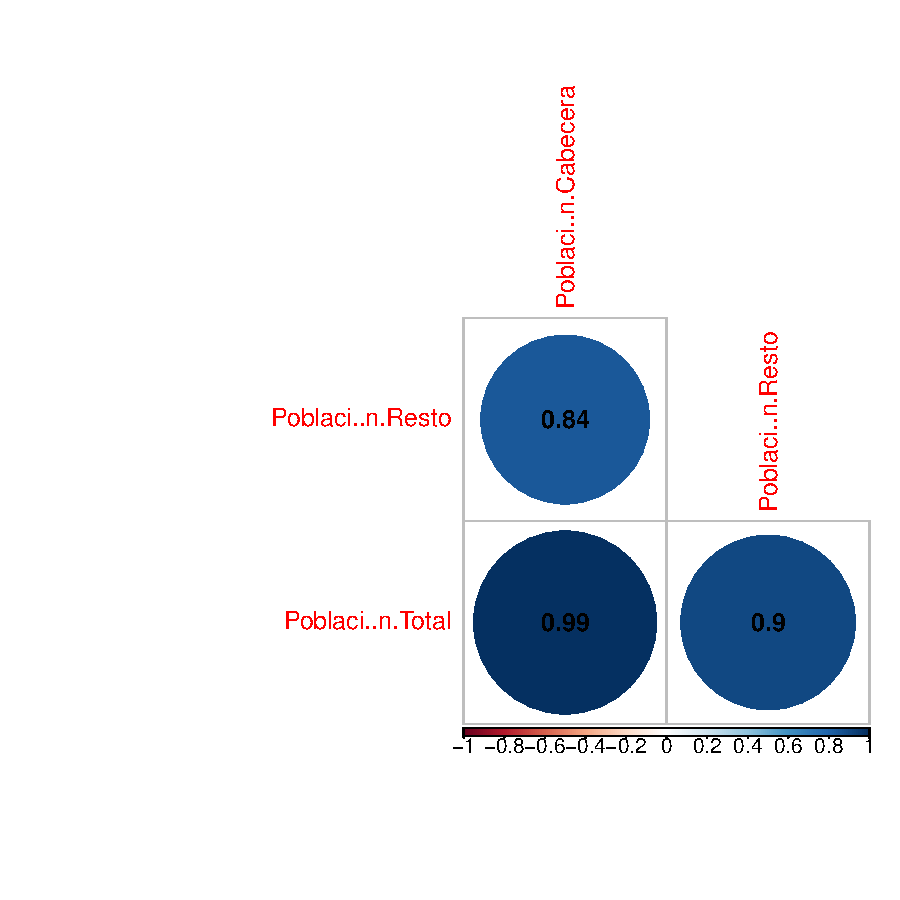
\includegraphics{ProyectoFinalJV-corrPlotX}


\end{adjustbox}
\caption{correlacion entre predictores}
\label{corrPlotX}
\end{figure}




%<<pcorre, echo=FALSE,fig=TRUE>>=
%# y la correlaci??n entre las variables independientes:
%#ver:
 % plot(colb[,explanans])


\clearpage

\section{Modelos de Regresion}






% Table created by stargazer v.5.2.2 by Marek Hlavac, Harvard University. E-mail: hlavac at fas.harvard.edu
% Date and time: Sat, Jul 07, 2018 - 18:46:51
\begin{table}[!htbp] \centering 
  \caption{Modelos de Regresion} 
  \label{regresiones} 
\begin{tabular}{@{\extracolsep{5pt}}lcc} 
\\[-1.8ex]\hline 
\hline \\[-1.8ex] 
 & \multicolumn{2}{c}{\textit{Dependent variable:}} \\ 
\cline{2-3} 
\\[-1.8ex] & \multicolumn{2}{c}{IDH} \\ 
\\[-1.8ex] & (1) & (2)\\ 
\hline \\[-1.8ex] 
 Cabecera.Ajustada & 0.013$^{***}$ & 0.031$^{***}$ \\ 
  & (0.004) & (0.007) \\ 
  & & \\ 
 Resto.Ajustada &  & $-$0.030$^{***}$ \\ 
  &  & (0.010) \\ 
  & & \\ 
 Constant & 0.634$^{***}$ & 0.766$^{***}$ \\ 
  & (0.055) & (0.065) \\ 
  & & \\ 
\hline \\[-1.8ex] 
Observations & 32 & 32 \\ 
R$^{2}$ & 0.238 & 0.425 \\ 
Adjusted R$^{2}$ & 0.212 & 0.385 \\ 
Residual Std. Error & 0.037 (df = 30) & 0.033 (df = 29) \\ 
F Statistic & 9.347$^{***}$ (df = 1; 30) & 10.706$^{***}$ (df = 2; 29) \\ 
\hline 
\hline \\[-1.8ex] 
\textit{Note:}  & \multicolumn{2}{r}{$^{*}$p$<$0.1; $^{**}$p$<$0.05; $^{***}$p$<$0.01} \\ 
\end{tabular} 
\end{table} 



\clearpage


\section{Exploracion Espacial}

 calculemos conglomerados de regiones colombianas usando toda la informacion de los indicadores. Como nuestras variables son ordinales utilizaremos un proceso de conglomeracion donde las distancia seran calculadas usando la medida 









\end{document}
